\documentclass[12pt]{article}
\usepackage[T1]{fontenc}
\usepackage{graphicx}
\usepackage{float}
\usepackage[polish]{babel}
\usepackage{amsmath}

\setlength{\textheight}{21cm}

\title{{\bf Zadanie nr 2 - Próbkowanie \\ i kwantyzacja}\linebreak
Cyfrowe Przetwarzanie Sygnałów}
\author{Jakub Wąchała, 216914 \and Radosław Grela, 216769}
\date{20.04.2020}

\begin{document}
\clearpage\maketitle
\thispagestyle{empty}
\newpage
\setcounter{page}{1}
\section{Cel zadania}
\label{cel}
Celem zadania jest oswojenie się z zagadnieniami dotyczącymi procesu konwersji analogowo-cyfrowej i cyfrowo analogowej sygnałów. Zadanie polega na implementacji wybranych wariantów konwersji, a także miar. 

\section{Wstep teoretyczny}
Program ten jest wzbogaconą o wybrane funkcjonalności wersją programu z zadania 1.
\subsection {Dodatkowo zaimplementowane warianty:}
\begin {enumerate}
\item Konwersja A/C - próbkowanie:
\begin {itemize}
 \item (S1) Próbkowanie równomierne
\end {itemize}
\item Konwersja A/C - kwantyzacja:
\begin {itemize}
\item (Q2) Kwantyzacja równomierna z zaokrąglaniem
\end {itemize}
\item Konwersja C/A - rekonstrukcja sygnału:

\begin {itemize}
\item (R1) Ekstrapolacja zerowego rzędu
\item (R2) Interpolacja pierwszego rzędu
\item (R3) Rekonstrukcja w oparciu o funkcję sinc
\end {itemize}
\end{enumerate}
\subsection {Dodatkowo zaimplementowane miary:}
\label{miary}
\begin {itemize}
\item  (C1) Błąd średniokwadratowy (MSE)
\item (C2) Stosunek sygnał - szum (SNR)
\item (C4) Maksymalna różnica (MD)
\end {itemize}
\begin{figure}[H]


\end{figure}

\section{Eksperymenty i wyniki}
Wykorzystując cztery rodzaje sygnałów (tj. sinusoidalny, trójkątny, sinusoidalny wyprostowany dwupołówkowo) przeprowadzimy konwersje analogowo - cyfrowe i cyfrowo - analogowe, a także zaprezentujemy rezultaty poszczególnych miar \ref{miary} . Kolorem czerwonym przedstawiony jest sygnał oryginalny, natomiast kolorem niebieskim jego konwersja.
\subsection{Sygnał sinusoidalny}
Celem eksperymentu jest przedstawienie wyników procesu konwersji analogowo - cyfrowej i cyfrowo analogowej dla sygnału sinusoidalnego.
Użyte parametry:
\begin{itemize}
\item amplituda: 15
\item okres: 5
\item czas początkowy: 0
\item czas trwania: 20
\end{itemize}
\subsubsection{Rezultat}
\begin{figure}[H]
\centering
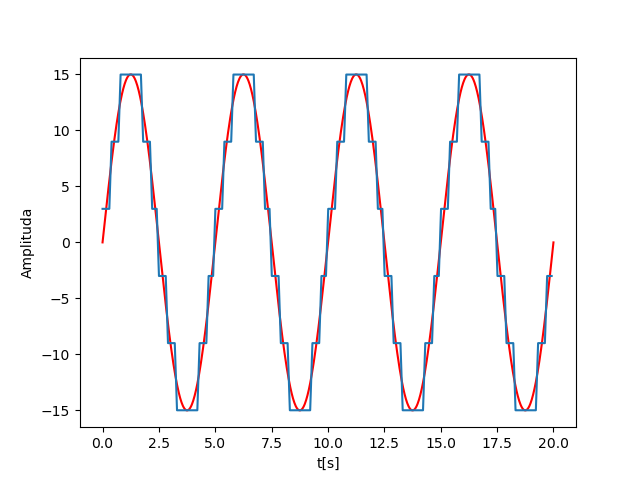
\includegraphics[scale=0.6]{1sinusKwantStopien5.png}
\caption{Wykres konwersji A/C (kwantyzacja równomierna z zaokrągleniem st. 5, 10hz, 200probek)}
\end{figure}

\begin{figure}[H]
\centering
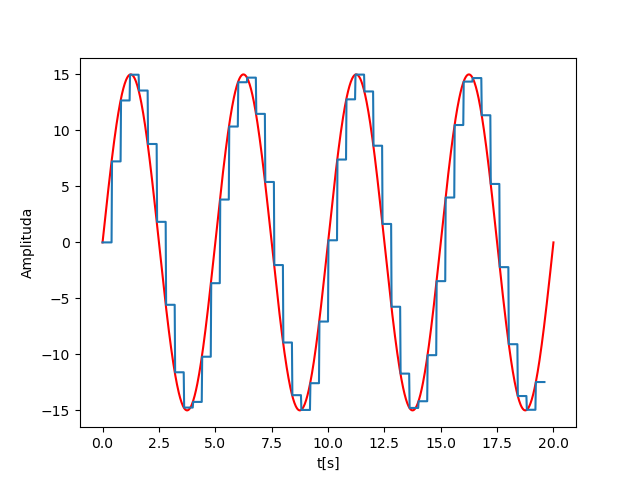
\includegraphics[scale=0.6]{2sinusEkstrapol0rzedu50.png}
\caption{Wykres konwersji C/A (ekstrapolacja zerowego rzędu, 50hz, 1000probek)}
\end{figure}

\begin{figure}[H]
\centering
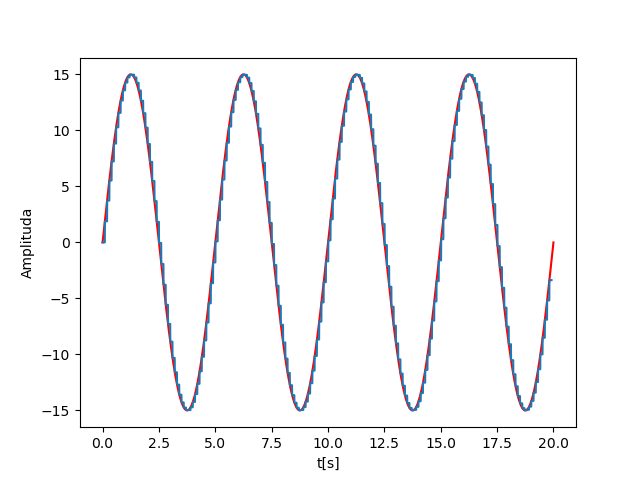
\includegraphics[scale=0.6]{2sinusEkstrapol0rzedu.png}
\caption{Wykres konwersji C/A (ekstrapolacja zerowego rzędu, 100hz, 2000probek)}
\end{figure}

\begin{figure}[H]
\centering
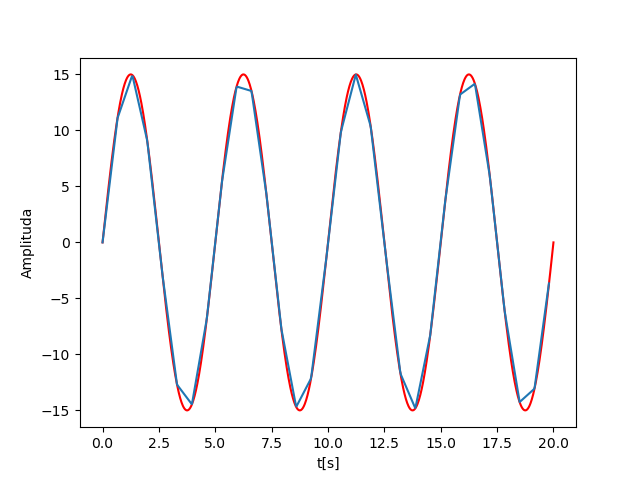
\includegraphics[scale=0.6]{33sinusinterpolacja1rzedu30.png}
\caption{Wykres konwersji C/A (interpolacja pierwszego rzędu 30hz,600probek)}
\end{figure}

\begin{figure}[H]
\centering
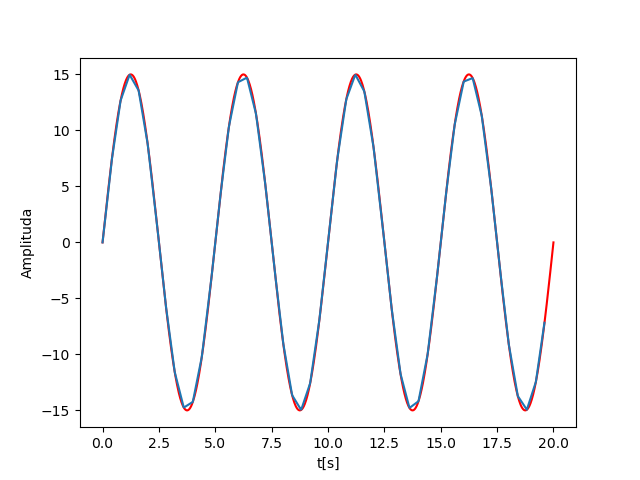
\includegraphics[scale=0.6]{34sinusinterpolacja1rzedu50.png}
\caption{Wykres konwersji C/A (interpolacja pierwszego rzędu, 50hz,1000probek)}
\end{figure}

\begin{figure}[H]
\centering
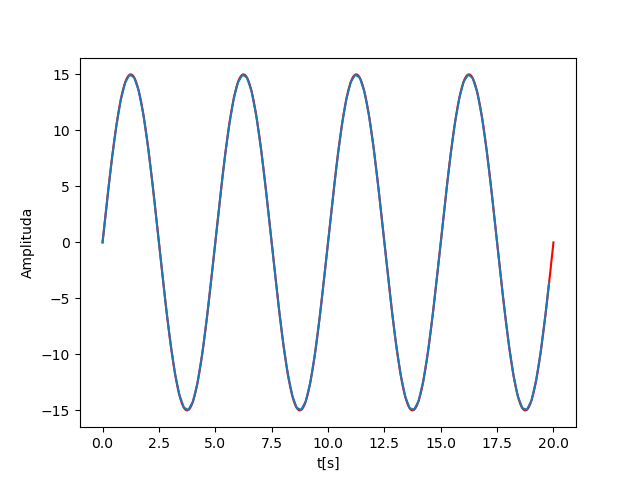
\includegraphics[scale=0.6]{34sinusinterpolacja1rzedu100.png}
\caption{Wykres konwersji C/A (interpolacja pierwszego rzędu, 100hz, 2000probek)}
\end{figure}

\begin{figure}[H]
\centering
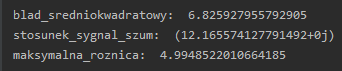
\includegraphics[scale=0.9]{333sinusMiarySt3.png}
\caption{Otrzymane miary dla sygnału sinusoidalnego, stopień 3, 200hz, 4000probek}
\end{figure}

\begin{figure}[H]
\centering
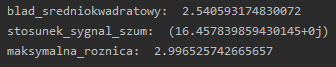
\includegraphics[scale=0.9]{3sinusMiary.png}
\caption{Otrzymane miary dla sygnału sinusoidalnego, stopień 5, 200hz, 4000probek}

\begin{figure}[H]
\centering
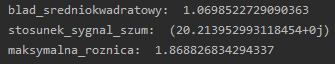
\includegraphics[scale=0.9]{333sinusMiarySt8.png}
\caption{Otrzymane miary dla sygnału sinusoidalnego, stopień 8, 200hz, 4000probek}
\end{figure}

\end{figure}
\subsection{Sygnał sinusoidalny wyprostowany dwupołówkowo}
Celem eksperymentu jest przedstawienie wyników procesu konwersji analogowo - cyfrowej i cyfrowo analogowej dla sygnału  sinusoidalnego wyprostowanego dwupołówkowo.
\label{syg2}
\subsubsection{Rezultat}


\begin{figure}[H]
\centering
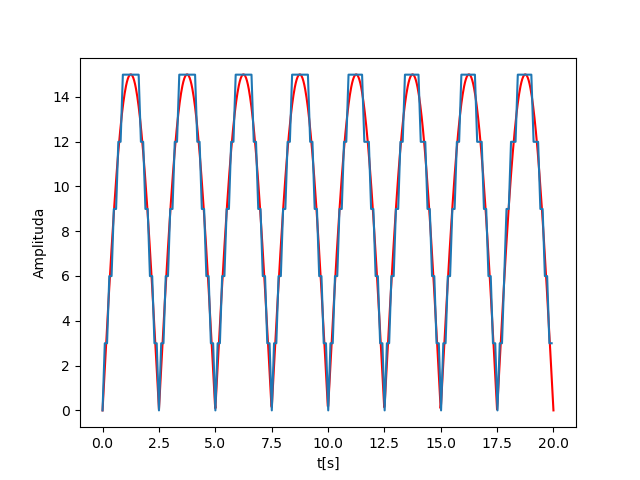
\includegraphics[scale=0.6]{10sygsinusDwuSin200kwantyzacja.png}
\caption{Wykres konwersji C/A (kwantyzacja równomierna z zaokrągleniem, 10hz, 200probek)}
\end{figure}

\begin{figure}[H]
\centering
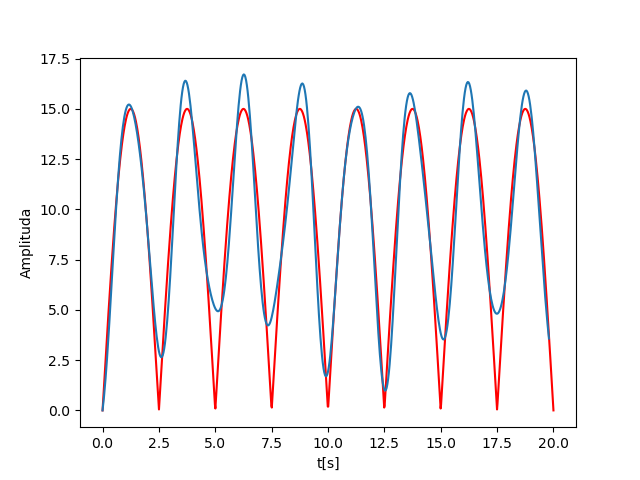
\includegraphics[scale=0.6]{11sygsinusDwuSin30czest.png}
\caption{Wykres konwersji C/A (rekonstrukcja w oparciu o funkcję sinus, 30hz, 600probek)}
\end{figure}

\begin{figure}[H]
\centering
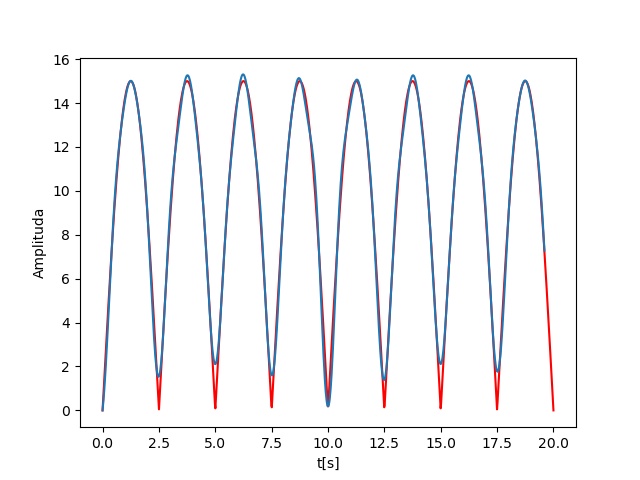
\includegraphics[scale=0.6]{122sygsinusDwuSin50czest.png}
\caption{Wykres konwersji C/A (rekonstrukcja w oparciu o funkcję sinus, 50hz, 1000probek)}
\end{figure}

\begin{figure}[H]
\centering
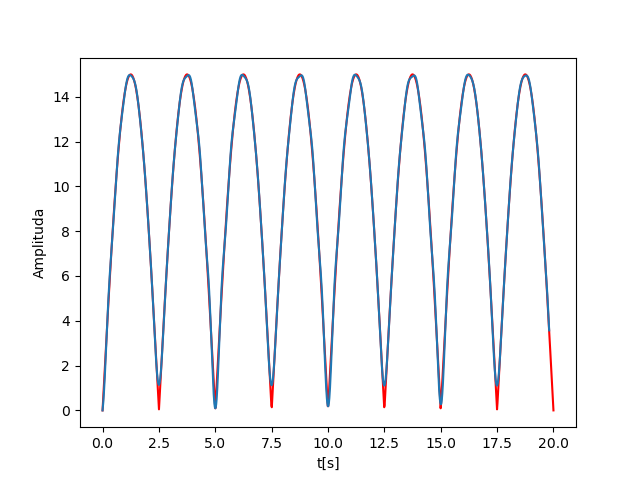
\includegraphics[scale=0.6]{12sygsinusDwuSin100czest.png}
\caption{Wykres konwersji C/A (rekonstrukcja w oparciu o funkcję sinus, 100hz, 2000probek)}
\end{figure}

\begin{figure}[H]
\centering
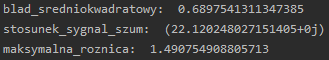
\includegraphics[scale=0.9]{444sinusDwuMiarySt5.png}
\caption{Otrzymane miary dla sygnału sinusoidalnego wyprostowanego dwupołówkowo, 200hz, stopień 5, 4000probek}
\end{figure}

\begin{figure}[H]
\centering
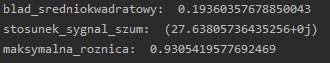
\includegraphics[scale=0.9]{444sinusDwuMiarySt8.png}
\caption{Otrzymane miary dla sygnału sinusoidalnego wyprostowanego dwupołówkowo, 200hz, stopień 8, 4000probek}
\end{figure}

\begin{figure}[H]
\centering
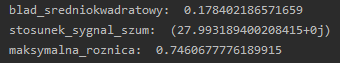
\includegraphics[scale=0.9]{444sinusDwuMiarySt10.png}
\caption{Otrzymane miary dla sygnału sinusoidalnego wyprostowanego dwupołówkowo, 200hz, stopień 10, 4000probek}
\end{figure}

\subsection{Sygnał trójkątny}
Celem eksperymentu jest przedstawienie wyników procesu konwersji analogowo - cyfrowej i cyfrowo analogowej dla sygnału trójkątnego.
Użyte parametry:
\begin{itemize}
\item amplituda: 15
\item okres: 5
\item czas początkowy: 0
\item czas trwania: 20
\end{itemize}
\subsubsection{Rezultat}
\begin{figure}[H]
\centering
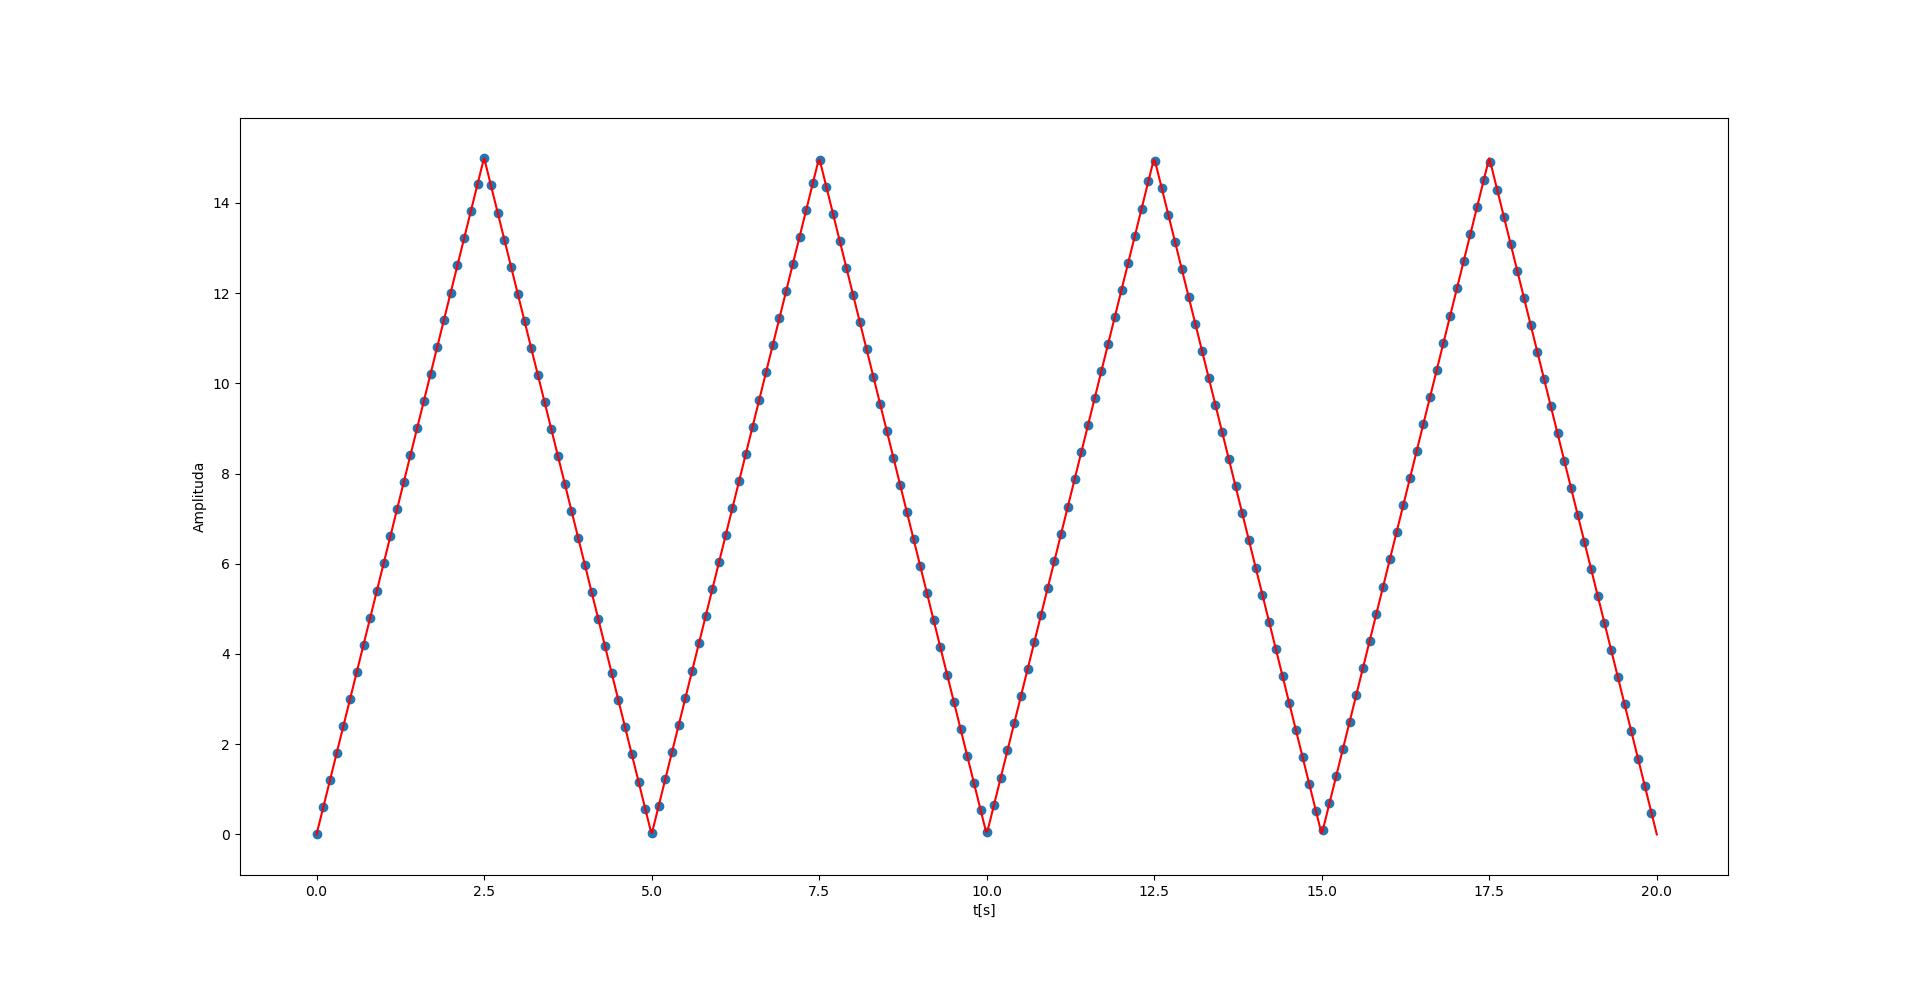
\includegraphics[scale=0.3]{7trojkatProbkowanie200.png}
\caption{Wykres konwersji A/C (próbkowanie, 10hz, 200probek)}
\end{figure}
\begin{figure}[H]
\centering
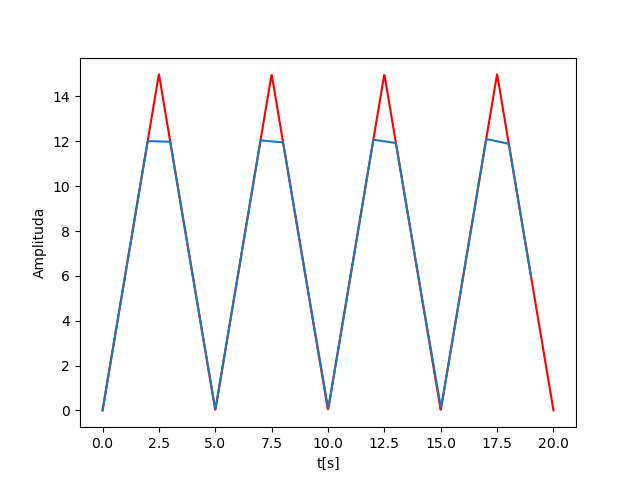
\includegraphics[scale=0.6]{8trojkatInterp1rzedu20.png}
\caption{Wykres konwersji C/A (interpolacja pierwszego rzędu 20hz,400probek)}
\end{figure}

\begin{figure}[H]
\centering
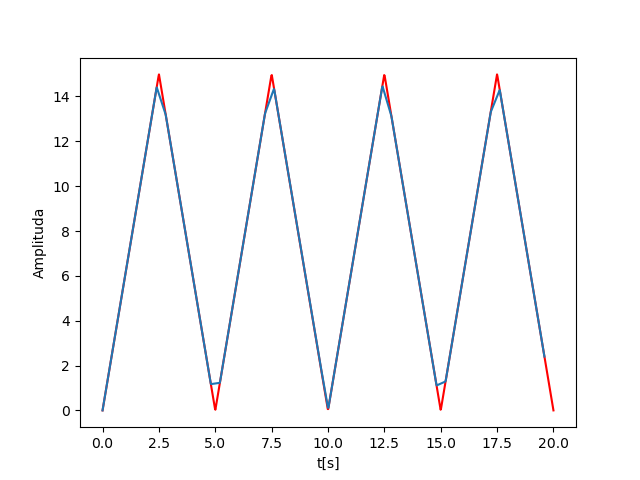
\includegraphics[scale=0.6]{8trojkatInterp1rzedu50.png}
\caption{Wykres konwersji C/A (interpolacja pierwszego rzędu, 50hz, 1000probek)}
\end{figure}

\begin{figure}[H]
\centering
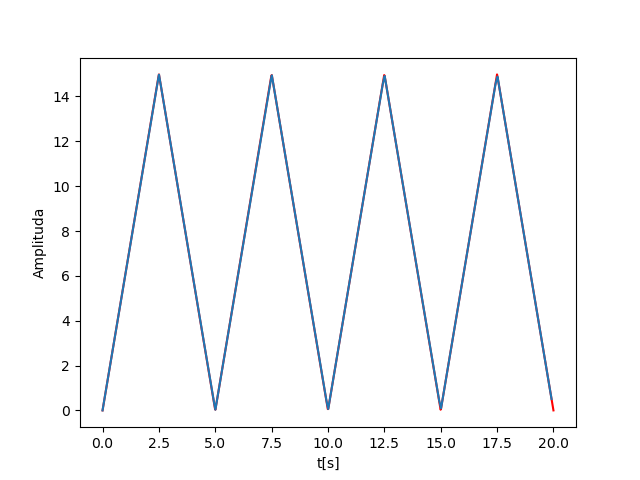
\includegraphics[scale=0.6]{8trojkatInterp1rzedu200.png}
\caption{Wykres konwersji C/A (interpolacja pierwszego rzędu, 200hz, 4000probek)}
\end{figure}

\begin{figure}[H]
\centering
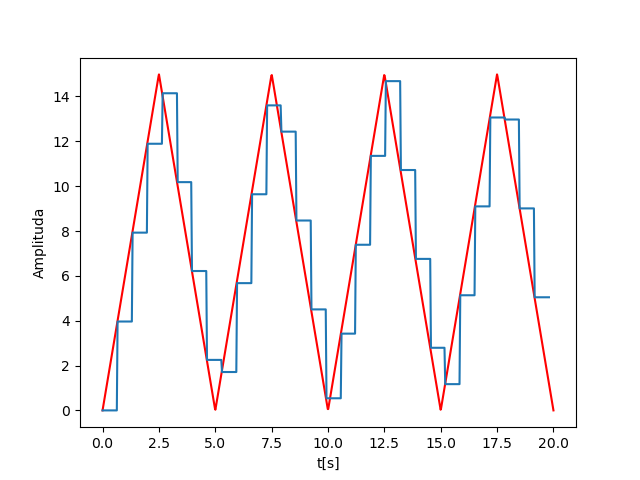
\includegraphics[scale=0.6]{77trojkatekstr0rzedu30.png}
\caption{Wykres konwersji C/A (ekstrapolacja zerowego rzędu, 30hz, 600probek)}
\end{figure}

\begin{figure}[H]
\centering
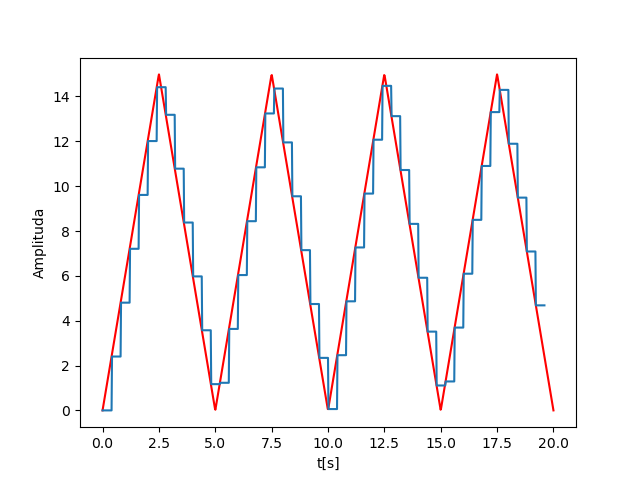
\includegraphics[scale=0.6]{77trojkatekstr0rzedu50.png}
\caption{Wykres konwersji C/A (ekstrapolacja zerowego rzędu, 50hz, 1000probek)}
\end{figure}

\begin{figure}[H]
\centering
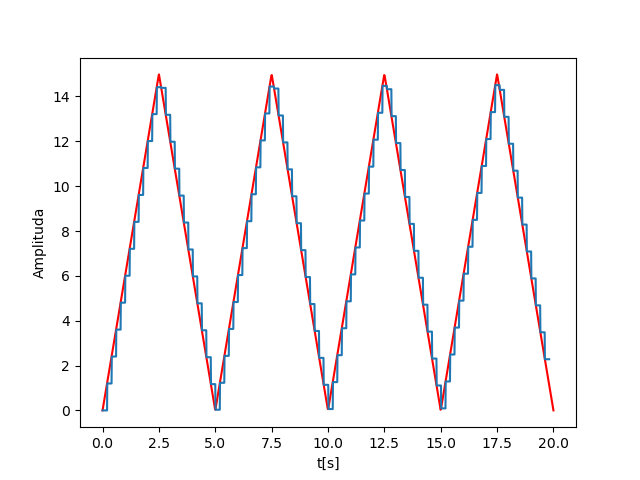
\includegraphics[scale=0.6]{77trojkatekstr0rzedu100.png}
\caption{Wykres konwersji C/A (ekstrapolacja zerowego rzędu, 100hz, 2000probek)}
\end{figure}


\begin{figure}[H]
\centering
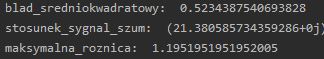
\includegraphics[scale=0.9]{555trojkatMiary20.png}
\caption{Otrzymane miary dla sygnału trójkątnego,5 stopień, 20hz, 400probek}
\end{figure}

\begin{figure}[H]
\centering
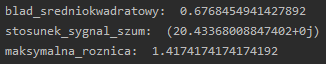
\includegraphics[scale=0.9]{555trojkatMiary50.png}
\caption{Otrzymane miary dla sygnału trójkątnego,5 stopień, 50hz, 1000probek}
\end{figure}

\begin{figure}[H]
\centering
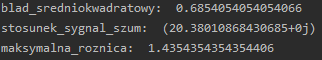
\includegraphics[scale=0.9]{555trojkatMiary100.png}
\caption{Otrzymane miary dla sygnału trójkątnego,5 stopień, 100hz, 2000probek}
\end{figure}

\begin{figure}[H]
\centering
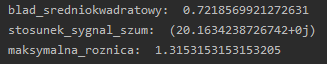
\includegraphics[scale=0.9]{9trojkatMiary.png}
\caption{Otrzymane miary dla sygnału trójkątnego,5 stopień, 200hz, 4000probek}
\end{figure}



\subsection{Zjawisko aliasingu}
Celem eksperymentu jest przedstawienie wyników zjawiska aliasingu w oparciu o samodzielnie wybrany zestaw funkcji. Aliasing jest to zniekształcenie (osłabienie lub wzmocnienie) sygnału powstałe w czasie jego próbkowania, które powstaje w wyniku niespełnienia założeń twierdzenia o próbkowaniu. Objawia się to powstaniem składowych o błędnych częstotliwościach (aliasów).
\newline
Do zobrazowania zjawiska wykorzystaliśmy funkcję sinus o częstotliwości 100hz, a następnie wykonaliśmy próbkowanie o częstotliwości 1000hz i zrekonstruowaliśmy sygnał w oparciu o funkcję sinus.

\begin{figure}[H]
\centering
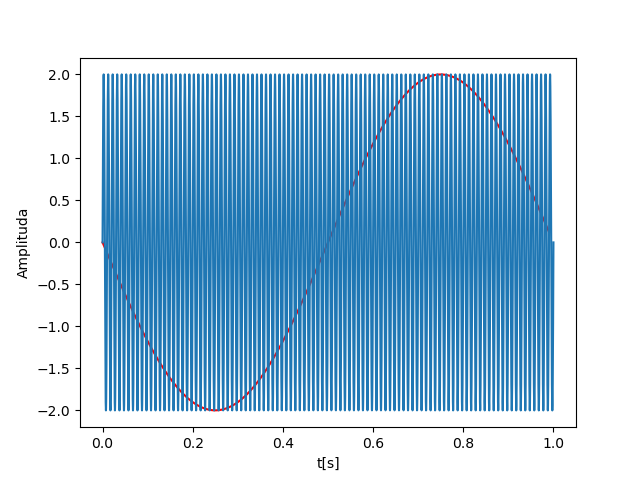
\includegraphics[scale=0.8]{666aliasing.png}
\caption{Otrzymane zjawisko aliasingu}
\end{figure}

\section{Wnioski}
\begin {itemize}
\item Prezentowane wyniki są dowodem na poprawne wykonanie zadania tj. poprawność konwersji A/C (kwantyzacji równomiernej z zaokrągleniem oraz próbkowania), C/A (interpolacji pierwszego rzędu, ekstrapolacji zerowego rzędu, rekonstrukcji w oparciu o funkcję sinus) wraz z ich miarami. Widzimy, że im większa częstotliwość (większa ilość próbek na sekundę) tym wykres zostaje zrekonstruowany w sposób bardziej dokładny.
\item W przypadku ekstrapolacji widać widoczne zniekształcenie w stosunku do sygnału oryginalnego ponieważ powstaje ona przy użyciu funkcji rect (prostokąt), przez co przybiera ona postać schodkową. Lepiej wygląda to w wypadku interpolacji.
\item Rekonstrukcja w opraciu o funkcję sinus jest dokładniejsza od ekstrapolacji zerowego rzędu (przyjmując, że porównujemy te same częstotliwości)
\item Im większy stopień kwantyzacji tym błąd oraz maksymalna różnica jest mniejsza
\end {itemize}


\begin{thebibliography}{0}
\bibitem{bib1}
\label{zad1}
\textit{Zadanie 2 - Próbkowanie i kwantyzacja} Cyfrowe Przetwarzanie Sygnału WIKAMP FTIMS\newline
\end{thebibliography}

\end{document}